\documentclass[a4paper]{article}

%------------------------------------------------------------
\usepackage[a4paper, total={6in, 9in}]{geometry}
\usepackage{amsmath, amssymb}
\usepackage{booktabs}
\usepackage{caption}
\usepackage{enumitem}
\usepackage{graphicx}
\usepackage{float}
\usepackage{inconsolata}
\usepackage{listings}
\usepackage{mathtools}
\usepackage{pstricks-add}
\usepackage{siunitx}
\usepackage[most]{tcolorbox}
\usepackage{tikz, pgfplots}
\usepackage{epstopdf} %converting to PDF
\usepackage{hyperref}
\usepackage{xfrac}

\usetikzlibrary{shapes.geometric}
\usetikzlibrary{arrows}

%------------------------------------------------------------
\graphicspath{{./fig/}}
\pgfplotsset{compat=1.13}
%------------------------------------------------------------
\setlength{\parindent}{0in}

\lstdefinestyle{C++}{
	language=C++,
	basicstyle=\ttfamily,
	keywordstyle=\color{blue}\ttfamily,
	stringstyle=\color{red}\ttfamily,
	commentstyle=\color{green}\ttfamily,
	morecomment=[l][\color{magenta}]{\#},
	showstringspaces=false
}

%------------------------------------------------------------
\newtcblisting[auto counter]{sexylisting}[2][]{sharp corners, 
    fonttitle=\bfseries, colframe=gray, listing only, 
    listing options={basicstyle=\ttfamily,language=C++}, 
    title=Listing \thetcbcounter: #2, #1}

%------------------------------------------------------------
\lstset{language=C++,
        basicstyle=\ttfamily,
        keywordstyle=\color{blue}\ttfamily,
        stringstyle=\color{red}\ttfamily,
        commentstyle=\color{green}\ttfamily,
        morecomment=[l][\color{magenta}]{\#},
        showstringspaces=false
}
%------------------------------------------------------------
\tikzstyle{block} = [draw, fill=blue!20, rectangle, 
    minimum height=3em, minimum width=3em]
\tikzstyle{sum} = [draw, fill=blue!20, circle, node distance=1cm]
\tikzstyle{input} = [coordinate]
\tikzstyle{output} = [coordinate]
\tikzstyle{pinstyle} = [pin edge={to-,thin,black}]

%------------------------------------------------------------
\newlength{\arrow}
\settowidth{\arrow}{\scriptsize$1000$}
\newcommand*{\myrightarrow}[1]{\xrightarrow{\mathmakebox[\arrow]{#1}}}

%------------------------------------------------------------

\begin{document}
\title{ENG252 Dynamics: Practical 1}
\author{Shane Reynolds}
\maketitle

\section{Introduction}
Consider an object, on Earth's surface, being launched into the air with an initial velocity at some angle with the horizontal. This very simple motion event is best analysed by considering it in two discrete parts: the object acceleration to the initial velocity; and the subsequent trajectory once the object is airborne.

\subsection{Acceleration to initial velocity}
If forces are denoted as $\boldsymbol{F}$, acceleration as $\boldsymbol{a}$, object mass as $m$, and time as $t$, then the object's acceleration can be modelled using the standard fare of Classical Mechanics: Newton's Second Law of Motion. This is shown in equation (1).
\begin{equation}
\sum \boldsymbol{F}(t) = m \boldsymbol{a}(t)
\end{equation}

The object could be accelerated along any curvilinear path, however, for the sake of simplicity let's assume the object is accelerated along a linear path. We note that acceleration can be formally defined as:
\begin{equation}
\boldsymbol{a} = \frac{d\boldsymbol{v}}{dt}
\end{equation}

Rearranging equation (1), substituting this into equation (2) and taking the integral of with respect to $t$, from the initial time, $t_0$, to the final time, $t$, yields the following:
\begin{equation}
\int_{\boldsymbol{v_0}}^{\boldsymbol{v}(t)} d\tilde{\boldsymbol{v}} = \frac{1}{m}\int_{t_0}^{t} \sum \boldsymbol{F}(\tau) d\tau
\end{equation}

Assuming that the force is constant over the duration of time $t-t_0$, equation (3) can be simplified as follows:
\begin{equation}
\boldsymbol{v}(t) = \boldsymbol{v_0} + \frac{(t-t_0)}{m} \sum \boldsymbol{F} 
\end{equation}

If the motion is planar then equation (4) can be decomposed according to a conveniently chosen two dimensional rectilinear orthonormal basis which describes the vector space. Typically, we use $\boldsymbol{\hat{e}_x}$, and $\boldsymbol{\hat{e}_y}$, such that $\boldsymbol{\hat{e}_y}$ is aligned with the force due to gravity, but any arrangement could be used.

\subsection{Trajectory once airborne}
Once airborne, there are typically only a few forces acting on the object: force due to gravity; and force opposing motion due to friction between the object and air. The force due to gravity can be calculated using another \textit{greatest hit} from the Classical Mechanics cannon: Newton's Law of Universal Gravitation. If we denote the mass of our object as $m$, the mass of the Earth as $M$, the Euclidean distance between their centres as $r$, and $G$ as a gravitational constant $6.674×10^{−11} \si{\newton(\meter\per\kilogram)^2}$ then the attractive force due to gravity is given by:
\begin{equation}
\boldsymbol{F} = G \frac{m M}{r^2}
\end{equation}

Assuming that the object trajectory does not take large excursions from the Earth's surface it is reasonable to assume that $r$ is constant, implying that the force due to gravity is also constant. If the force due to air resistance is assumed to be negligible, then the object is said to be undermoving constant acceleration $g$, which is approximately $9.81\si{\meter\per\second^2}$. A 2D orthonormal basis describing the vector space of the motion, say $\boldsymbol{\hat{e}_x}$ and $\boldsymbol{\hat{e}_y}$, can be aligned such that $\boldsymbol{\hat{e}_y}$ is parallel to the direction of $g$. Under these assumptions the equations of motion describing the object trajectory can be seen in Table 1.
\begin{table}[h]
	\centering
	\caption{Equations of motion governing a projectile under constant gravitation acceleration assumption, with negliglible air resistance}
	\begin{tabular}{ll}
		\toprule
		Equations of motion $(x)$ & Equations of motion $(y)$\\
		\midrule
		$s_x(t) = (s_0)_x + (v_0)_x t$ & $s_y(t) = (s_0)_y + (v_0)_y t -\frac{1}{2}gt^2 $ \\
		$v_x(t) = (v_0)_x$ & $v_y(t) = (v_0)_y - gt$ \\
		$a_x(t) = 0$ & $a_y(t) = -g$ \\
		\bottomrule
	\end{tabular}
\end{table}

The parametric displacement equations in Table 1 describe the trajectory of the object as it travels through the air. Letting $s_x(t) = x$ we can rearrange the horizontal displacement equation as:
\begin{equation}
t = \frac{x - (s_0)_x}{(v_0)_x} = \frac{1}{(v_0)_x}x - \frac{(s_0)_x}{(v_0)_x}
\end{equation}

Substituting this into the vertical displacement equation, and letting $s_y(t) = y$, we see that:
\begin{equation}
y = (s_0)_y + (v_0)_y \bigg(\frac{1}{(v_0)_x}x - \frac{(s_0)_x}{(v_0)_x} \bigg) -\frac{1}{2}g \bigg(\frac{1}{(v_0)_x}x - \frac{(s_0)_x}{(v_0)_x} \bigg)^2
\end{equation}

Expanding equation (7) and simplifiying results illustrates the trajectory shape in the 2D plane is quadratic.


\subsection{Scope}
The scope of this practical is to apply a force to a small electric car, accelerating it along a short linear track. Once the car leaves the track it will follow a quadratic trajectory. The time taken to travers 0.1$\si{\meter}$ at the end of the linear track will be measures, as well as the horizontal distance travelled by the car. The average velocity will be used as a proxy for instantaneous launch velocity, and a predicted horizontal distance will be calculated. The practical will conclude with a discussion around the reliability of predictive calculations when estimating real life projectile motion scenarios.

\newpage

\section{Setup}
A model electric car, shown in Figure 1, is accelerated along a 1.4$\si{\meter}$ track by an electric dc motor. Two metal strips along the track length have a 12$\si{\volt}$ voltage potential difference applied whcih power the dc motor when two metal tabs on the car's underside touch the track conductors. The track, shown in Figure 2, is proped up at a known angle with an aluminium strut. Upon reaching the track termination the car is lauched into the air, at which point it continues a parabolic trajectory until it lands on a mat. The horizontal distance from the track end to the position where the car landed is measured.
\begin{figure}[h]
	\begin{minipage}[t]{0.45\textwidth}
		\centering
		\frame{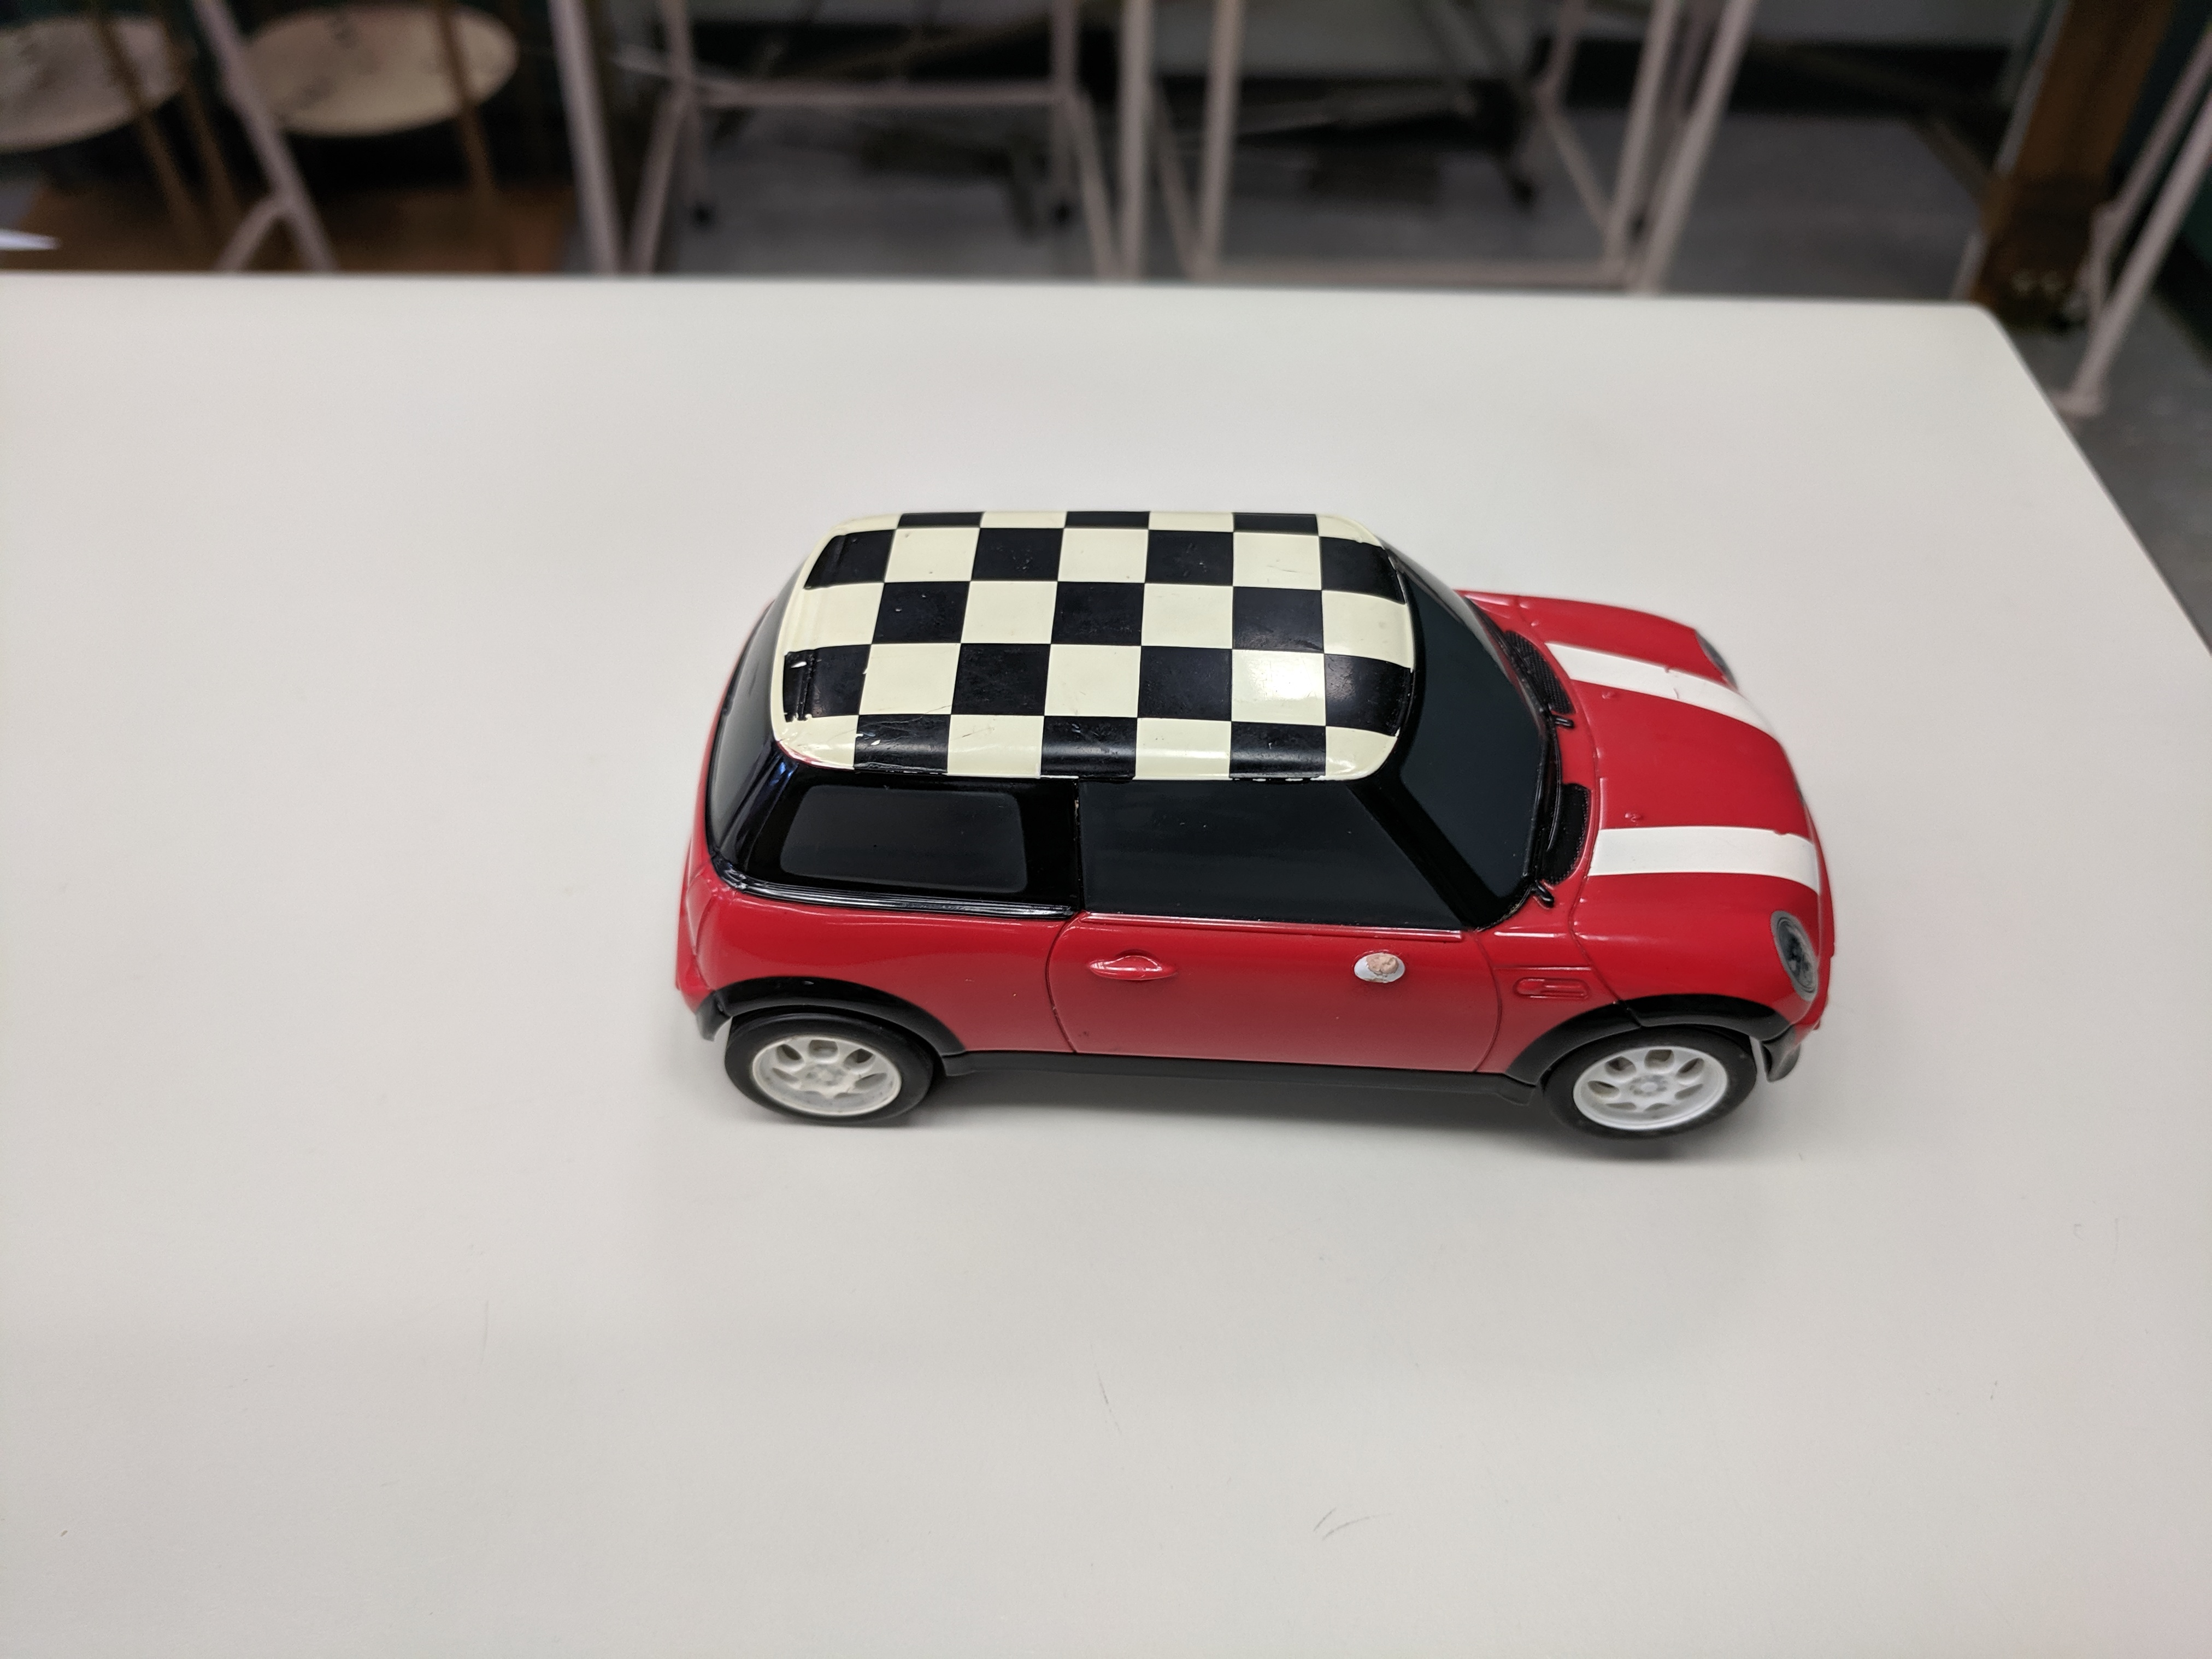
\includegraphics[scale=0.05]{fig1}}
		\caption{The car used for the practical.}
	\end{minipage}
	\hspace{1cm}
	\begin{minipage}[t]{0.45\textwidth}
		\centering
		\frame{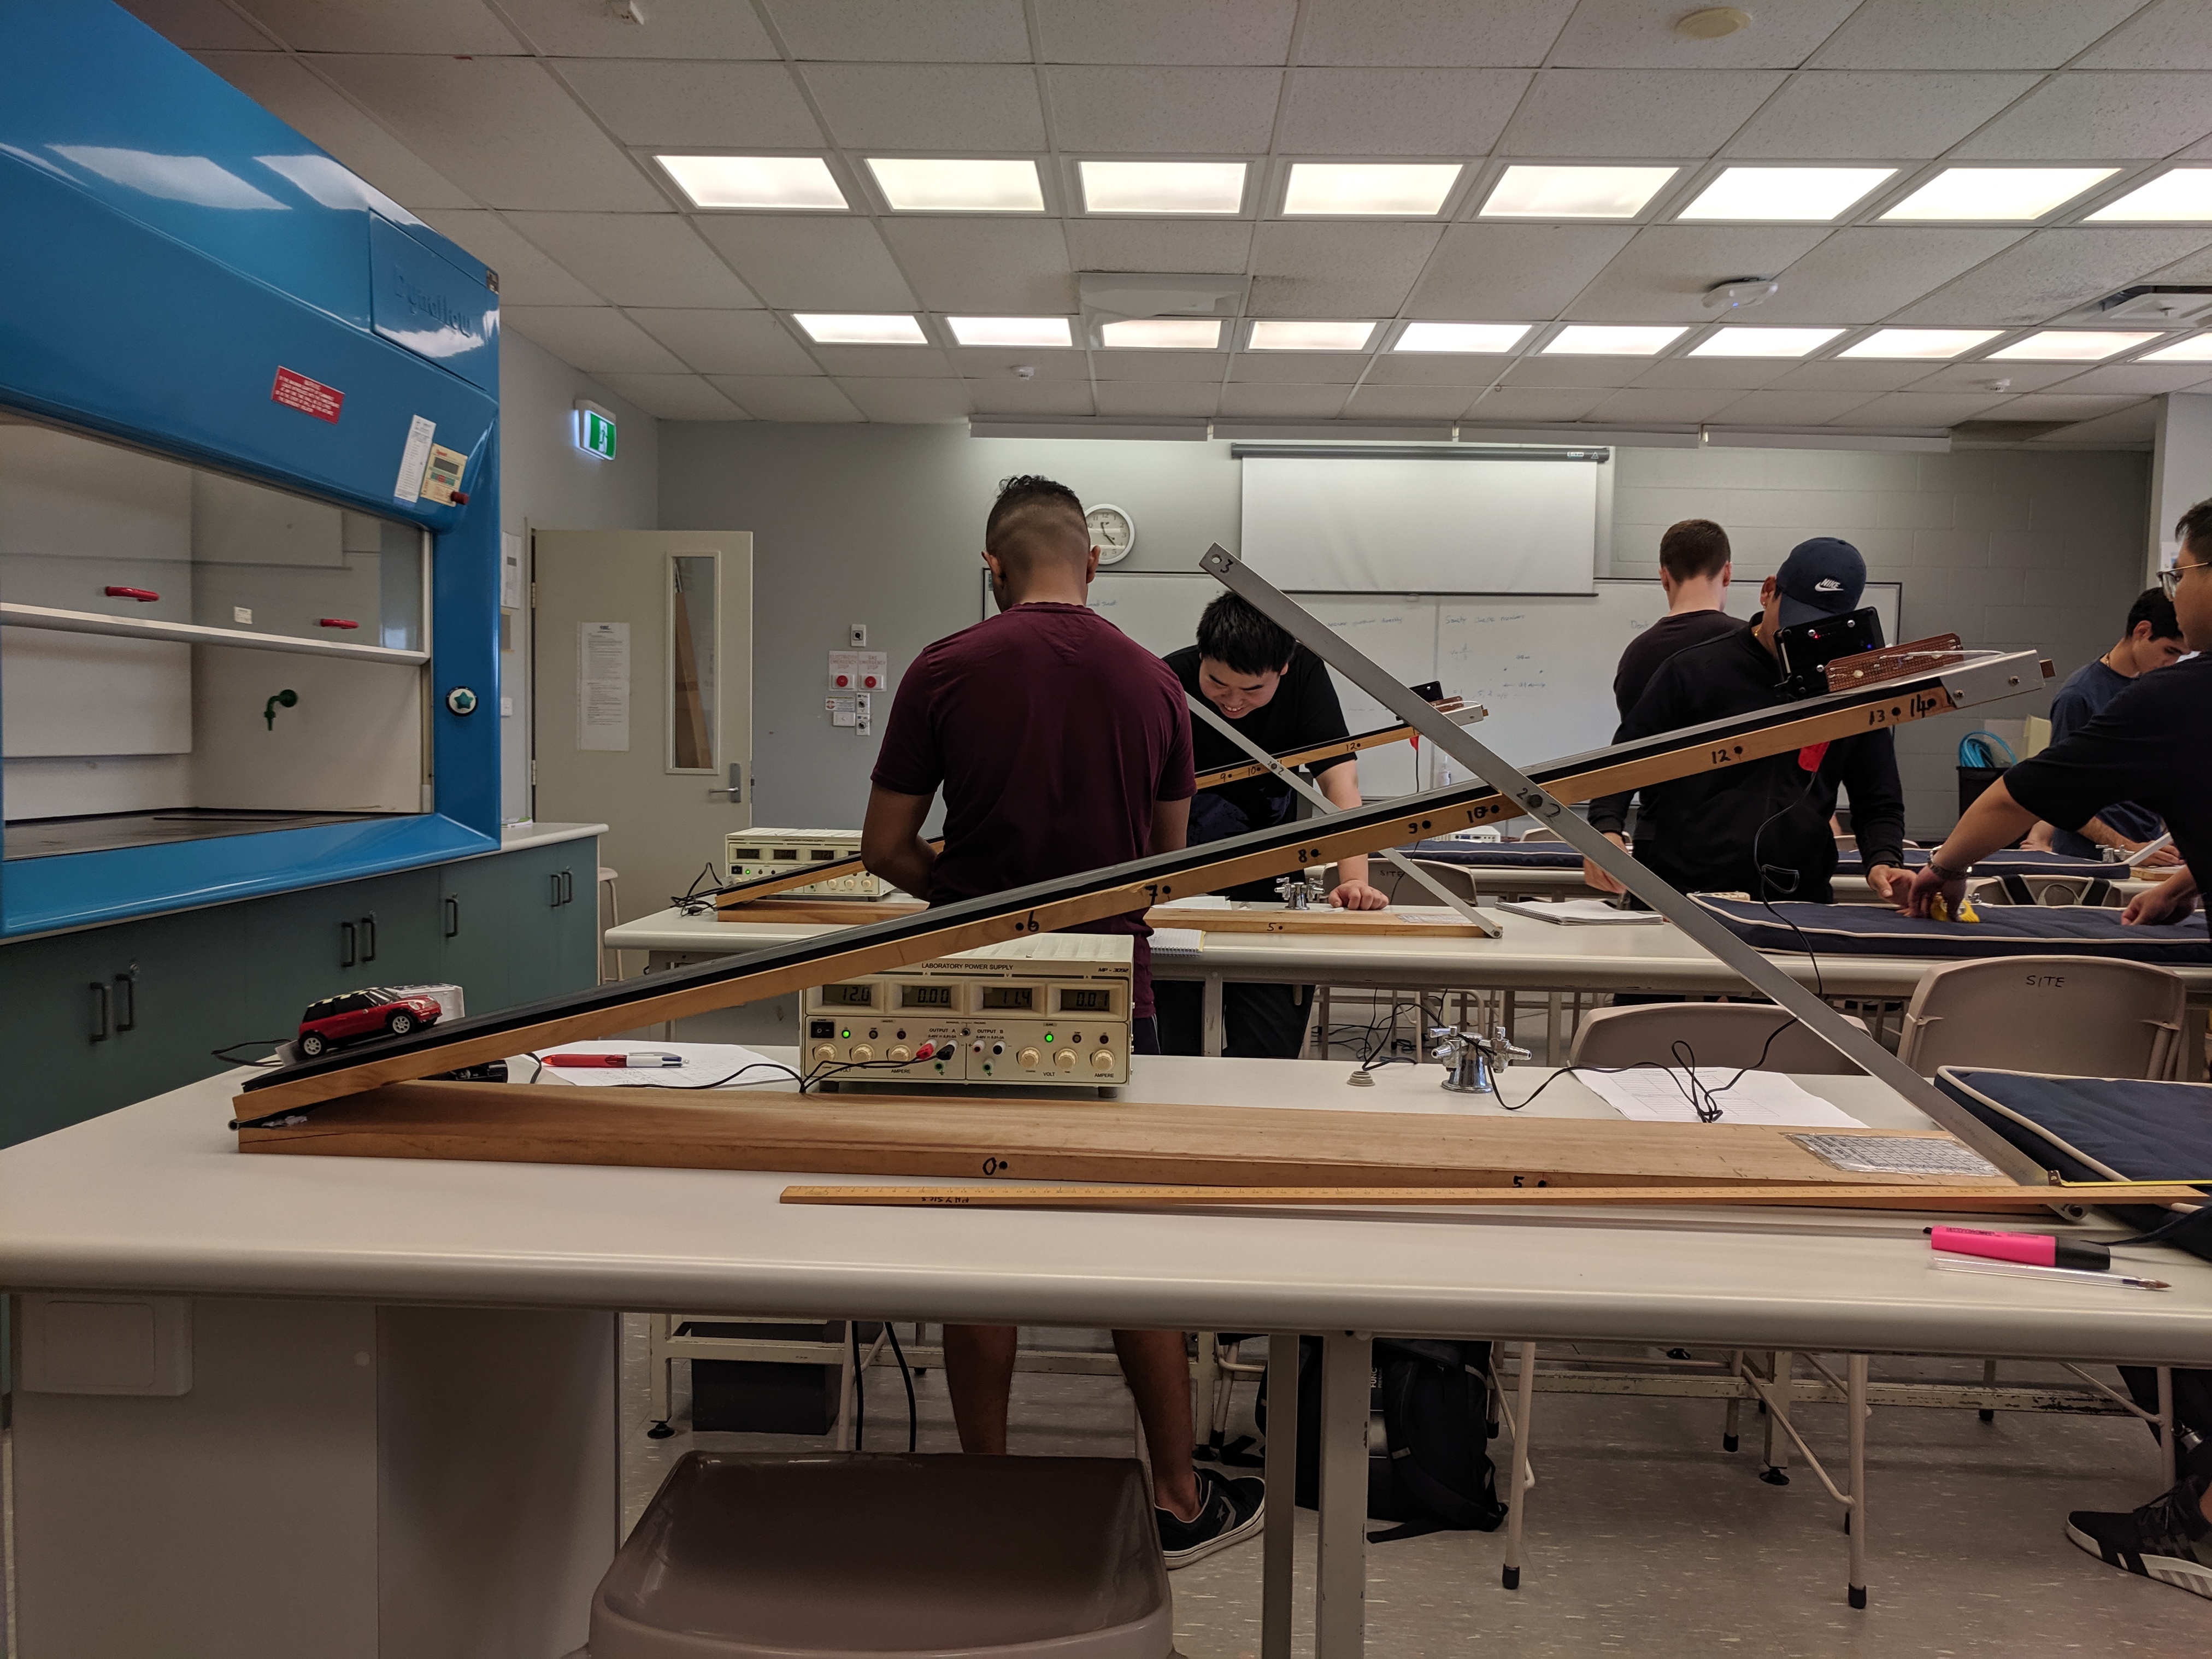
\includegraphics[scale=0.05]{fig2}}
		\caption{The track used for the practical - this setup was located in the right rear corner of the laboratory.}
	\end{minipage}
\end{figure}

Towards the end of the track, a short 0.1$\si{\meter}$ section of the track is fit with a timer which trips on and off again as the car passes through. This can be seen in Figure 3. The timer provides a measurement of the time taken for the car to traverse the 0.1$\si{\meter}$ section of the track, allowing for the calculation of an approximate launch velocity as the car leaves the track.
\begin{figure}[h]
	\centering
	\frame{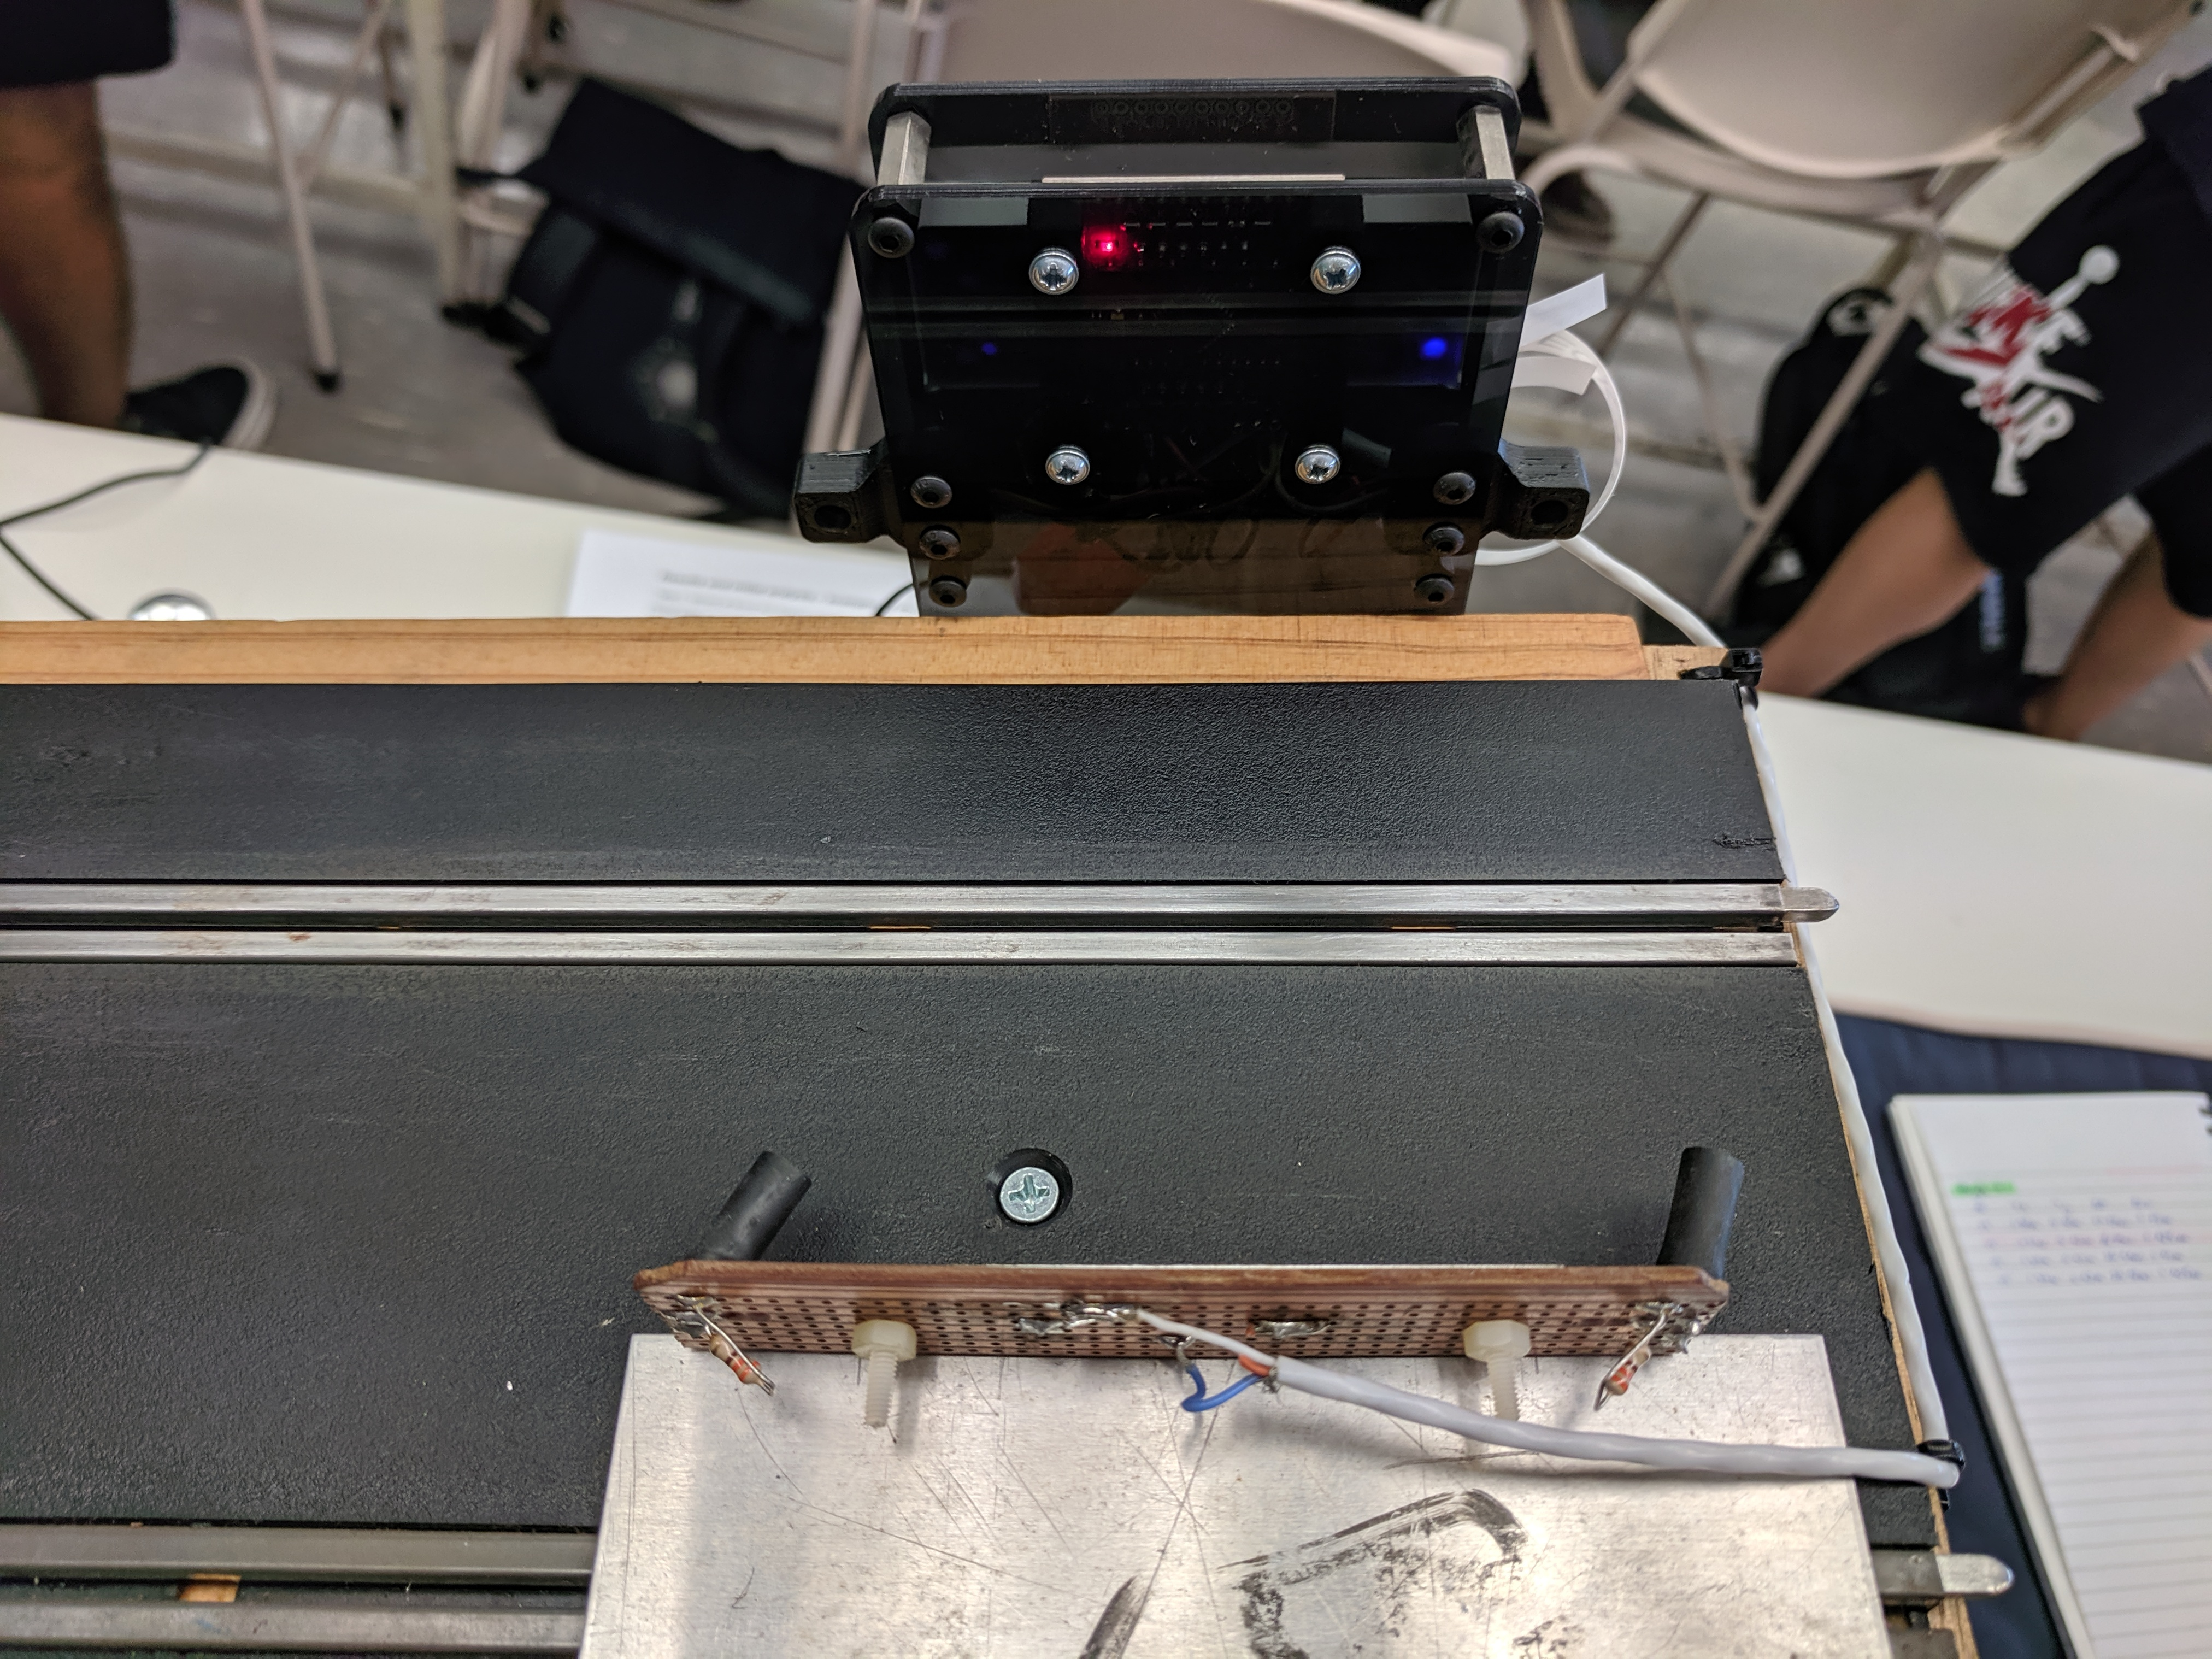
\includegraphics[scale=0.05]{fig3}}
	\caption{The short linear section (0.1 meter) of the track which trips a timer on and off as the car passes through - this allows the user to approximate a launch velocity for the vehicle.}
\end{figure}

\newpage

\section{Results}
Four different angles were selected to provide coverage of the launch angle range available. The angles, in radians, were: $\sfrac{\pi}{4}$, $\sfrac{7\pi}{36}$, $\sfrac{5\pi}{36}$, and $\sfrac{\pi}{12}$. Setting the track launch angle was not straight forward. Supporting calculations were made to confirm the launch angle. Measurements of the horizontal distance along the track base were taken. This length is shown as $T_x$ in Figure 4. Similarly, the launch height was also measured - this is shown as $T_y$ in Figure 4. To confirm the launch angle a calculation was made using basic trigonometry:
\begin{equation}
\theta = \arctan\bigg(\frac{T_y}{T_x}\bigg)
\end{equation}

The calculated results can be seen in Table 2. The car was launched off the ramp, at each angle, four times. Each launch saw two measurements taken: the horizontal distance, $(s_f)_x$, the car travelled from the end of the ramp; the time taken, $\delta t$ ,  for the car to pass a distance of $0.1\si{\meter}$ at the end of the ramp. The tabulared results can be seen in Tables 3, 4, 5, and 6 below.

\begin{figure}[h]
	\begin{minipage}{0.45\textwidth}
		\centering
		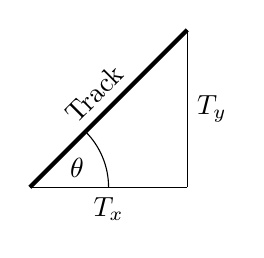
\begin{tikzpicture}
		\draw (0,0) -- node[below]{$T_x$} (2,0);
		\draw (2,0) -- node[right]{$T_y$} (2,2);
		\draw[line width=0.55mm] (2,2) -- node[above, rotate=45]{Track} (0,0);
		\draw (1,0) arc (0:45:1);
		\node at (0.6,0.25) {$\theta$};
		\end{tikzpicture}
		\caption{The measurements $T_x$ and $T_y$ form a right angle triangle allowing for the calculation of $\theta$ using trigonometry.}
	\end{minipage}
	\hspace{1cm}
	\begin{minipage}{0.45\textwidth}
		\centering
		\captionof{table}{Calculated angles, using trigonometry, are approximately the listed angles on the track setup.}
		\begin{tabular}{rrl}
			\toprule
			$T_x \ [\si{\meter}]$ & $T_y \ [\si{\meter}]$ & $\theta \ [\si{\radian}]$\\
			\midrule
			1.01 & 1.01 & $0.785 \approx \sfrac{\pi}{4}$\\
			1.16 & 0.83 & $0.621 \approx \sfrac{7\pi}{36}$\\
			1.275 & 0.64 & $0.465 \approx \sfrac{5\pi}{36}$\\
			1.37 & 0.42 & $0.297 \approx \sfrac{\pi}{12}$\\
			\bottomrule
		\end{tabular}
	\end{minipage}
\end{figure}

\begin{figure}[h]
	\begin{minipage}{0.45\textwidth}
		\centering
		\captionof{table}{Measurements of $\delta t$ and $(s_f)_x$ taken for the a launch angle of $\sfrac{\pi}{4}$}
		\begin{tabular}{crr}
			\toprule
			Trial No. & $\delta t \ [\si{\milli\second}]$ & $(s_f)_x \ [\si{\meter}]$\\
			\midrule
			1 & 48.01 & 1.025\\
			2 & 46.70 & 0.985\\
			3 & 44.60 & 1.010\\
			4 & 46.42 & 1.040\\
			\midrule
			Average & 46.43 & 1.015 \\
			\bottomrule
		\end{tabular}
	\end{minipage}
	\hspace{1cm}
	\begin{minipage}{0.45\textwidth}
		\centering
		\captionof{table}{Measurements of $\delta t$ and $(s_f)_x$ taken for the a launch angle of $\sfrac{7\pi}{36}$}
		\begin{tabular}{crr}
			\toprule
			Trial No. & $\delta t \ [\si{\milli\second}]$ & $(s_f)_x \ [\si{\meter}]$\\
			\midrule
			1 & 35.66 & 1.470\\
			2 & 35.16 & 1.485\\
			3 & 33.68 & 1.520\\
			4 & 34.04 & 1.525\\
			\midrule
			Average & 34.64 & 1.500 \\
			\bottomrule
		\end{tabular}
	\end{minipage}
\end{figure}

\begin{figure}[h]
	\begin{minipage}{0.45\textwidth}
		\centering
		\captionof{table}{Measurements of $\delta t$ and $(s_f)_x$ taken for the a launch angle of $\sfrac{5\pi}{36}$}
		\begin{tabular}{crr}
			\toprule
			Trial No. & $\delta t \ [\si{\milli\second}]$ & $(s_f)_x \ [\si{\meter}]$\\
			\midrule
			1 & 30.34 & 1.590\\
			2 & 30.39 & 1.540\\
			3 & 29.73 & 1.570\\
			4 & 29.94 & 1.575\\
			\midrule
			Average & 30.10 & 1.569 \\
			\bottomrule
		\end{tabular}
	\end{minipage}
	\hspace{1cm}
	\begin{minipage}{0.45\textwidth}
		\centering
		\captionof{table}{Measurements of $\delta t$ and $(s_f)_x$ taken for the a launch angle of $\sfrac{\pi}{12}$}
		\begin{tabular}{crr}
			\toprule
			Trial No. & $\delta t \ [\si{\milli\second}]$ & $(s_f)_x \ [\si{\meter}]$\\
			\midrule
			1 & 27.27 & 1.450\\
			2 & 26.79 & 1.425\\
			3 & 26.94 & 1.410\\
			4 & 26.92 & 1.405\\
			\midrule
			Average & 26.98 & 1.423 \\
			\bottomrule
		\end{tabular}
	\end{minipage}
\end{figure}

\newpage

\section{Calculations}
Equation (4) relies on a known force profile, applied to the object, to determine the launch velocity reached at the linear track termination. With some effort, the force could be found using detailed information about the electric motor dynamics and torque speed characterisitcs. A simpler method of calculating initial launch velocity magnitude would be to calculate average velocity over a short distance towards the track termination, and use this value as an approximate. If the short distance is denoted as $\Delta s$, and the time taken to traverse this distance is $\delta t$, then average velocity is calculated as:
\begin{equation}
v_{avg} = \frac{\Delta s}{\delta t}
\end{equation}

As outlined in Section 2, a small device of approximately $0.1\si{\meter}$ in length measures the time taken for the car to traverse this distance. Letting $\Delta s = 0.1\si{\meter}$, and using the average times calculated in Tables 3, 4, 5, and 6 for $\delta t$, we can calculate the approximate launch velocity for each of the ramp angles. The results of these calculations can be found in Table 7.
\begin{figure}[h]
	\begin{minipage}{0.45\textwidth}
		\centering
		\captionof{table}{Approximate launch velocity}
		\begin{tabular}{cr}
			\toprule
			Angle $(\theta)$ & Velocity $(|\boldsymbol{v_0}|)$ \\
			$[\si{\radian}]$ & $[\si{\meter\per\second}]$ \\
			\midrule
			$\sfrac{\pi}{4}$ & 2.15 \\
			$\sfrac{7\pi}{36}$ & 2.89 \\
			$\sfrac{5\pi}{36}$ & 3.32 \\
			$\sfrac{\pi}{12}$ & 3.71 \\
			\bottomrule
		\end{tabular}
	\end{minipage}
	\hspace{0.25cm}
	\begin{minipage}{0.52\textwidth}
		\centering
		\begin{tikzpicture}
			\begin{axis}
				[
				axis y line = middle,
				axis x line = middle,
				domain=0:5,
				xmin=0,xmax=6,
				ymin=0,ymax=5,
				ticks=none
				]
				\addplot[blue]{-0.5*(x*x-4*x-5)};
				\addplot[thick, red, ->, domain=0:1]{2.5+2*x};
				\addplot[domain=0:1]{2.5};
			\end{axis}
			\node[left] (a) at (0,2.8) {$(s_0)_y$};
			\node[below] (b) at (5.8,0) {$(s_f)_x$};
			\node[red,above] (b) at (1.3,5) {$\boldsymbol{v_0}$};
			\node[above] (b) at (0.32,2.82) {$\theta$};
		\end{tikzpicture}
		\caption{As the car leaves linear track it follows a parabolic trajectory with an initial height of $(s_0)_y$, and a final horizontal distance of $(s_0)_x$.}
	\end{minipage}
\end{figure}

Suppose the initial velocity $\boldsymbol{v_0}$, launch angle $\theta$, and launch height $(s_0)_y$ are known. The initial velocity can be decomposed into $x$ and $y$ components as follows:
\begin{align}
(v_0)_x &= |\boldsymbol{v_0}|\cos(\theta)\\
(v_0)_y &= |\boldsymbol{v_0}|\sin(\theta)
\end{align}

To find a prediction of horizontal distance, $(\hat{s}_f)_x$, at the point of projectile impact we employ the known equation of motion for $s_x(t)$ shown in Table 1. In order to calculate $(\hat{s}_f)_x$, we first need to determine the time taken for the object to collide with the ground. This is obtained with the equation for vertical displacement, $s_y(t)$, also shown in Table 1. Specifically, we are interested in the case when $s_y(t) = 0$. This yields the following:
\begin{equation}
0 = (s_0)_y + (v_0)_y t - \frac{1}{2}gt^2
\end{equation}

Multiplying equation (12) throughout by 2, and solving using the quadratic formula yields:
\begin{equation}
t = \frac{2(v_0)_y \pm \sqrt{4(v_0)_y^2 + 8g(s_0)_y}}{2g}
\end{equation} 

Noting that $2(v_0)_y < \sqrt{4(v_0)_y^2 + 8g(s_0)_y}$ and $t>0$ we can discard one solution. Hence, when $(s_y(t) = 0)$, we note that:
\begin{equation}
t = \frac{2(v_0)_y + \sqrt{4(v_0)_y^2 + 8g(s_0)_y}}{2g}
\end{equation}

To find predicted horizotal distance ${(\hat{s}_x)_f}$ we substitute the expression for time in (14) to the equation of horizontal displacement, $s_x(t)$, from Table 1. This will gives us the following:
\begin{equation}
(\hat{s}_f)_x = (s_0)_x + \frac{(v_0)_x}{2g} \bigg[2(v_0)_y + \sqrt{4(v_0)_y^2 + 8g(s_0)_y}\bigg]
\end{equation}

Noting that, by design, our coordinate system assignment ensures that $(s_0)_x = 0$, hence, equation (15) simplifies to:
\begin{equation}
(\hat{s}_f)_x = \frac{(v_0)_x}{2g} \bigg[2(v_0)_y + \sqrt{4(v_0)_y^2 + 8g(s_0)_y}\bigg]
\end{equation}

Equation (16) has been applied to each of the four launch angles. The important parameters here are: $\theta$, $\boldsymbol{v_0}$, and $(s_0)_y$. The calculation results can be seen in Table 8.
\begin{table}[h]
	\centering
	\caption{Calculation of the horizontal distance travelled.}
	\begin{tabular}{rrrrrr}
		\toprule
		$\theta$ ($\si{\radian}$) & $\boldsymbol{v_0}$ ($\si{\meter\per\second}$) & $(v_0)_x$ ($\si{\meter\per\second}$) & $(v_0)_y$ ($\si{\meter\per\second}$) & $(s_0)_y$ ($\si{\meter}$) & $(\hat{s}_f)_x$ ($\si{\meter}$)\\
		\midrule
		$\sfrac{\pi}{4}$ & 2.15 & 1.52 & 1.52 & 1.01 & 0.97 \\
		$\sfrac{7\pi}{36}$ & 2.89 & 2.37 & 1.66 & 0.83 & 1.45 \\
		$\sfrac{5\pi}{36}$ & 3.32 & 3.01 & 1.40 & 0.64 & 1.60 \\
		$\sfrac{\pi}{12}$ & 3.71 & 3.58 & 0.96 & 0.42 & 1.45 \\
		\bottomrule
	\end{tabular}
\end{table}

To deterimine the final velocity prior to impact we note that we need to determine the velocity magnitude $|\boldsymbol{v_f}|$ and the angle with the horizontal $\alpha$. Given we know $(v_x)_f$, and $(v_y)_f$, these variables can be determined using Pythogoras' theorem and basic trigonometry as follows:
\begin{align}
|\boldsymbol{v_f}| &= \sqrt{(v_f)_x^2 + (v_f)_y^2}\\
\alpha &= -\arctan\bigg(\frac{(v_f)_y^2}{(v_f)_x^2}\bigg)
\end{align} 

The horizontal velocity never changes since the only force acting on the car while airborne is gravity, which is orthogonal to the horizontal component of the velocity. Hence, we can write that:
\begin{equation}
(v_f)_x = (v_0)_x
\end{equation}

To find the vertical velocity on impact, the equation of vertical velocity, $v_y(t)$, can be used - this is shown in Table 1. The time of impact has already been expressed in equation (14). Using this with the $v_y(t)$, we can show that the horizontal welocity is given by:
\begin{equation}
(v_f)_y = (v_0)_y - \frac{1}{2} \bigg[2(v_0)_y + \sqrt{4(v_0)_y^2 + 8g(s_0)_y}\bigg]
\end{equation}

This simplifies to the following:
\begin{equation}
(v_f)_y = - \frac{1}{2} \sqrt{4(v_0)_y^2 + 8g(s_0)_y}
\end{equation}

Given that values for the initial horizontal and vertical velocities, $(v_0)_x$ and $(v_0)_y$, respectively; and the launch height, $(s_0)_y$, are known then magnitude and angle with the horizontal of the impact velocity can be calculated using equations (21), (17), and (18). The results of these calculations can be found in Table 9.

\begin{table}[h]
	\centering
	\caption{Calculation of the magnitide and angle with the horizontal of final velocity on impact.}
	\begin{tabular}{rrrrrrr}
		\toprule
		$\theta$ ($\si{\radian}$) & $|\boldsymbol{v_0}|$ ($\si{\meter\per\second}$) & $(v_0)_x$ ($\si{\meter\per\second}$) & $(v_0)_y$ ($\si{\meter\per\second}$) & $(s_0)_y$ ($\si{\meter}$) & $|\boldsymbol{v_f}|$ ($\si{\meter\per\second}$) & $\alpha$ (degree)\\
		\midrule
		$\sfrac{\pi}{4}$ & 2.15 & 1.52 & 1.52 & 1.01 & 4.95 & -72.06 \\
		$\sfrac{7\pi}{36}$ & 2.89 & 2.37 & 1.66 & 0.83 & 4.96 & -61.53 \\
		$\sfrac{5\pi}{36}$ & 3.32 & 3.01 & 1.40 & 0.64 & 4.86 & -51.69 \\
		$\sfrac{\pi}{12}$ & 3.71 & 3.58 & 0.96 & 0.42 & 4.69 & -40.21 \\
		\bottomrule
	\end{tabular}
\end{table}

\newpage

\section{Discussion}
The calculated distance, $(\hat{s}_f)_x$, was not a reliable predictor of the actual horizontal distance travelled, $(s_f)_x$. The results comparing calculated and actual values can be seen in Table 10. The table also shows the error between predicted and actual, $(\hat{s}_f)_x - (s_f)_x$, denoted as $\epsilon$. Finally, in the last column in Table 10, $\epsilon$ is considered as a percentage of the actual measured distance, $\sfrac{\epsilon}{(s_x)_f}$.

\begin{table}[h]
	\centering
	\caption{Calculated horizontal distance travelled, compared to the actual distance travelled.}
	\begin{tabular}{rrrrr}
		\toprule
		$\theta$ ($\si{\radian}$) &  $(\hat{s}_f)_x$ ($\si{\meter}$) & $(s_f)_x$ ($\si{\meter}$) & $\epsilon$ ($\si{\meter}$) & \% error\\
		\midrule
		$\sfrac{\pi}{4}$ & 0.97 & 1.015 & -0.048 & -4.75 \\
		$\sfrac{7\pi}{36}$ & 1.45 & 1.500 & -0.049 & -3.27 \\
		$\sfrac{5\pi}{36}$ & 1.60 & 1.569 & 0.032 & 2.03 \\
		$\sfrac{\pi}{12}$ & 1.45 & 1.423 & 0.032 & 2.23 \\
		\bottomrule
	\end{tabular}
\end{table}

The data shows that at higher launch angles the prediction appears to under estimate the actual distance, and at lower angles the prediction appears to over estimate the actual distance. Prediction error severity seems to mitigate as the launch angle becomes lower with the biggest prediction error at a launch angle of $\sfrac{\pi}{4}$ with a value -5$\si{\centi\meter}$ and the smallest at a launch angle of $\sfrac{\pi}{12}$ with value +3$\si{\centi\meter}$. The error mitigation trend is also shown in the \% error field. Errors range from approximately 2\% to 5\% of the actual value travelled, which is material in size - this is the principal reason for concluding that calculated horizontal distances in this analysis are not reliable. Explaining the root cause of the observed errors is difficult because, although there are only a small number of data points, the error seems to be following a trend which would rule out systematic errors from measurement devices like the timer at the end of the track. Furthermore, a 5\% error seems to be unreasonaly large to ascribe to air resistance forces. Another cause of the errors could be put down to human error in measurement, however, the expectation would be that these errors would be stochasitic in nature and not following a trend. Further measurements of existing angles, and new angles, would help to determine if the trend is concidence or if there is some other factor involved. \\ 

The voltage applied to the track is a constant 12$\si{\volt}$. The two conductors on the car's underside touch the track and complete the circuit, which powers the small electric dc motor mounted in the car. Torque speed characteristics are different depending on the dc motor circuit topology, however, most arrangements see torque fall away as the motor speed increase. Since torque is providing force to accelerate the car, we can conclude that acceleration is not constant over the track length.\\

The analysis undertaken here assumes that the car is a point mass, as it travels through the air. The actual dynamics of the car in flight sees the body of the vehicle rotating around the mass centroid of the vehicle, causing it to tumble when airborne. In spite of this our point mass assumption remains reasonable since the car is not in contact with any other body while airborne, meaning that the vehicle centroid is approximately the point mass. 

\section{Conclusion}

\bibliography{my_bib}
\bibliographystyle{ieeetr}

\end{document}